\documentclass[a4paper, 11pt]{article}

% Fonts 
\usepackage{opensans}
\usepackage{amsfonts}
\usepackage{montserrat}
\usepackage{amsmath}

\usepackage[mathrm=sym]{unicode-math}

\setmainfont{opensans}
\setmathfont{Fira Math}

\newfontfamily{\montserrateb}{Montserrat SemiBold}
\newfontfamily{\montserratb}{Montserrat Bold}
\newfontfamily{\montserrat}{Montserrat Regular}
\newfontfamily{\montserratl}{Montserrat Light}
\DeclareMathAlphabet{\mathcal}{OMS}{cmbrs}{m}{n}

% \autoref
\usepackage{hyperref}

% Use for [H] option for figures to force in text placement
\usepackage{float}

% Captioning figures
\usepackage{caption}

% Subfigures
\usepackage{subcaption}

% For extending contents beyond margins
\usepackage{scrextend}

% For tables \midrule ect
\usepackage{booktabs}

% Colours
\usepackage[table,xcdraw]{xcolor}
\definecolor{accentcolor}{HTML}{6332a8}

% Change label in enumerate 
\usepackage{enumitem}

% Section settings
\usepackage{titlesec}
\titleformat{\section}
{\LARGE\montserrateb}
{\thesection.}{0.5em}{}

\titleformat{\subsection}
{\large\montserratb}
{\thesubsection.}{0.5em}{}

% Adjust document dimensions
\ExecuteOptions{a4paper}
\addtolength{\oddsidemargin}{-3cm} 
\addtolength{\evensidemargin}{-3cm}
\addtolength{\topmargin}{-3cm} 
\addtolength{\textwidth}{6cm}
\addtolength{\textheight}{4.5cm}
\addtolength{\textheight}{1.5cm}
\addtolength{\headsep}{-0.5cm}
% \addtolength{\footskip}{-1cm}
\parindent0pt
\parskip=4pt



\usepackage{matlab-prettifier}
\usepackage{graphicx}
\usepackage{mdframed}

% Creates coloured title box
\newcommand{\thetop}[5]{
    \begin{addmargin}[\oddsidemargin]{\oddsidemargin}
        \colorbox{#5}{\color{white}
          \hbox to \paperwidth{
            \vbox {
              \begin{center}
                {\large\montserratl #1}\\
                \vspace{4pt}
                {\huge\montserratb #2}\\
                {\montserratb #3}\\
                \vspace{-0.5em}
                \rule{20em}{1pt}     
      
                {\large\montserratl 
                    #4
                }
              \end{center}
            }
          }
        }
    \end{addmargin}
}

\newcommand{\NN}{\mathbb{N}}
\newcommand{\ZZ}{\mathbb{Z}}
\newcommand{\RR}{\mathbb{R}}
\newcommand{\CC}{\mathbb{C}}
\newcommand{\dydt}{\frac{dy}{dt}}
\newcommand{\dxdt}{\frac{dx}{dt}}
\def\set#1{\left\{ #1 \right\}}
\def\eval#1#2{\left\ #1\right|_{#2}}
\begin{document}
\thetop{Robert Christie}{MATHS 340}{S1 2023}{Assignment 1\\Due: 1-08-2023}{accentcolor}

\section*{Q1}
\begin{enumerate}[label=(\alph*)]
  \item
        We can see that the surface $S$, is defined implicitly $f(x,y,z)=0$ where $f:\RR^3\to \RR$ is continuously differentiable (as it is a polynomial). Thus, we can see that as $(a,b,c)=(1,2,1)$ is a surface point, the tangent plane is given by:
        \begin{align*}
          0 & = \frac{\partial f}{ \partial x}(a,b,c)(x-a) +
          \frac{\partial f}{ \partial y}(a,b,c)(y-b) +
          \frac{\partial f}{ \partial z}(a,b,c)(z-c)         \\
            & = 2a(x-a) + 4b(y-b) - 10c(z-c)                 \\
            & = 2(x-1) + 8(y-2) -10(z-1)                     \\
          % & = 2x - 2 + 8y -16 -10z + 10                    \\
            & = 2x  + 8y  -10z -8
        \end{align*}

        % We see that $f(1,2,1)=0$, thus the point is indeed on the surface. We can use the formula given in lectures for the tangent plane to an implicit surface $S$ defined by $f(x,y,z)=0$
  \item MATLAB code for producing plot:
        \lstset{columns=flexible}
        \lstset{keepspaces=true}
        \begin{mdframed}[backgroundcolor=black!10]
          \begin{lstlisting}[style=Matlab-editor]
syms x y z
f = x.^2 + 2*y.^2 - 5*z.^2 - 4; % Implicit eq for surface
x0 = [1;2;1];                   % Point for tangent plane

% Implicit function for tangent plane
t = subs(jacobian(f, [x, y, z]), [x, y, z], x0.')*([x;y;z]-x0);

% Shadding and colouring
colormap(bone); lighting gouraud; shading interp;
fimplicit3(f);  % Plot implicit surface
hold on         % Overlay both surfaces
fimplicit3(t);  % Plot the x0 tangent plane (Twice for colouring trick)
fimplicit3(t, "FaceColor", [0.9, 0.1, 0.1], "FaceAlpha", 0.5); 

% Label the plot
xlabel('x'); ylabel('y'); zlabel('z');
title("Surface x^2 + 2y^2 - 5z^2 = 4 with [1 2 1]^T tangent plane")
view([-238.75 6.89])
  \end{lstlisting}
        \end{mdframed}
        Resulting plot shown in \autoref{fig:plot}.

        \begin{figure}
          \centering
          \begin{minipage}[t]{0.6\textwidth}
            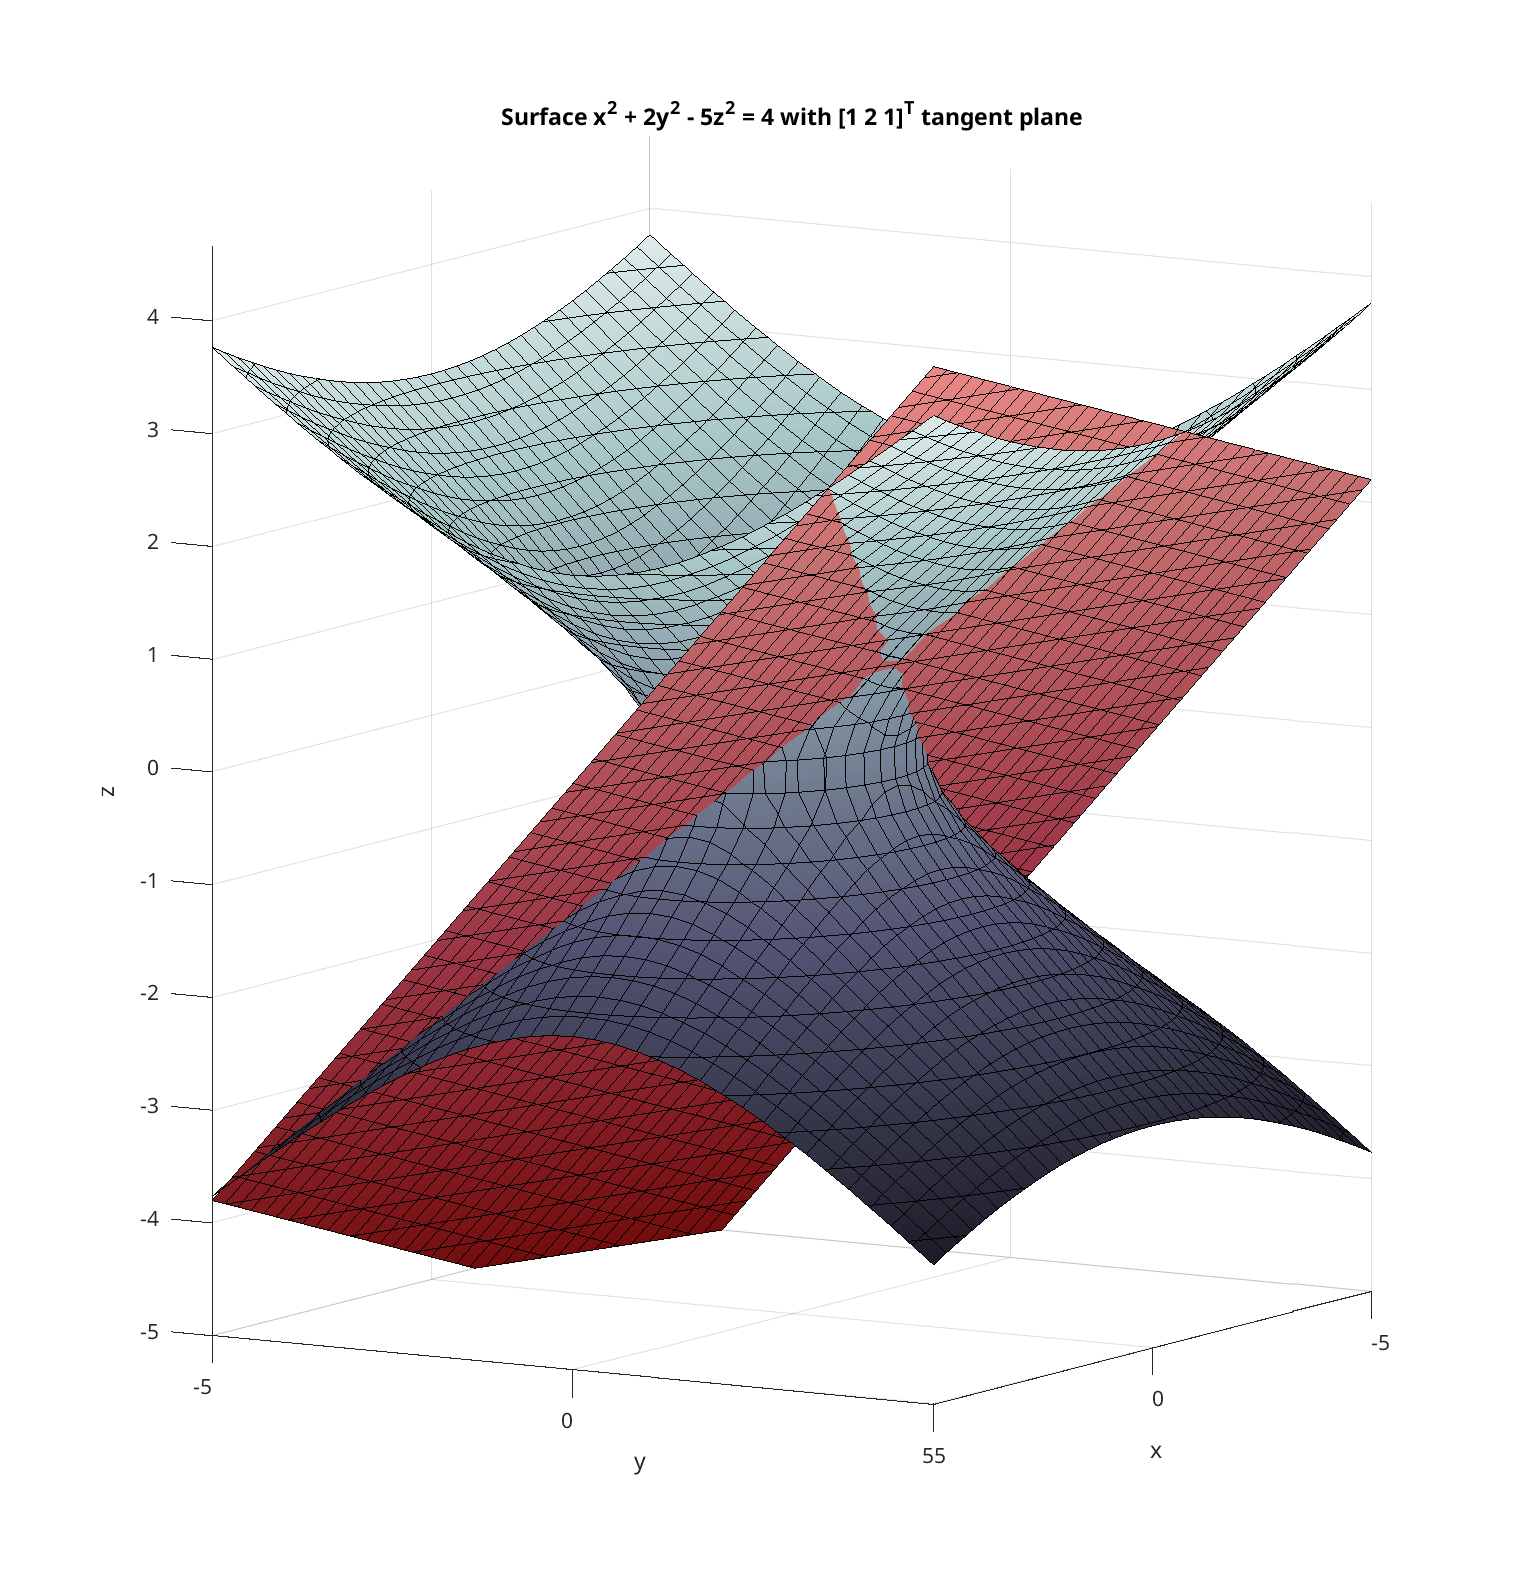
\includegraphics[width=\textwidth]{images/graph.eps}
            \caption{ Plot of the tangent plane for the point $[1,2,1]^T$ for the surface implicitly defined by $x^2+2y^2-5z^2=4$}
            \label{fig:plot}

          \end{minipage}
        \end{figure}


  \item
        We are considering a surface defined by a function $f(x,y,z)=0$, evaluating $f(0,0,1)=-9\neq 0$, thus the point does not lie on the surface. Since there is no surface at this point to be tangent to, it does not make sense to ask for the tangent plane at this point.

        % We could still use $f$ to find a plane at this point from the partial derivatives of $f$, however, this plane is not determined by the surface, it is determined by the choice of implicit function $f$, any plane passing through this point could match this definition by choosing a different $f$ that gives the same surface.




\end{enumerate}

\def\pp#1#2{\dfrac{\partial#1}{\partial#2}}
\def\dd#1#2{\dfrac{d#1}{d#2}}


\section*{Q2}
\begin{enumerate}[label=(\alph*)]
  \item Consider the function $\zeta: \begin{bmatrix}
            u \\ v
          \end{bmatrix} \mapsto \begin{bmatrix}
            x \\ y
          \end{bmatrix}$. From the definitions given we know:
        $$
          \zeta: \begin{bmatrix}
            u \\v
          \end{bmatrix} \mapsto \begin{bmatrix}
            ve^u \\
            ve^{-u}
          \end{bmatrix}
        $$
        Thus we find that:
        $$
          D\zeta = \left[ \begin{array}{c|c}\pp\zeta u& \pp\zeta v\end{array} \right] = \begin{bmatrix}
            ve^u     & e^u    \\
            -ve^{-u} & e^{-u} \\
          \end{bmatrix}
        $$
        The columns of $D\zeta$ give us a moving frame of basis vectors, which we normalise to give unit vectors:

        \begin{align*}
          e_u & = \frac{
          \begin{bmatrix}
            ve^u \\
            -ve^{-u}
          \end{bmatrix}
          }{
          \sqrt{v^2e^{2u} + v^2e^{-2u}}
          }
          = \frac{
            \begin{bmatrix}
              e^u \\
              -e^{-u}
            \end{bmatrix}}{
            \sqrt{e^{2u} + e^{-2u}}
          }
          = \begin{bmatrix}
              \sqrt{\frac{e^{2u}}{e^{2u} + e^{-2u}}} \\
              -\sqrt{\frac{e^{-2u}}{e^{2u} + e^{-2u}}}
            \end{bmatrix}
          = \begin{bmatrix}
              \sqrt{\frac{1}{\frac{e^{2u} + e^{-2u}}{e^{2u}}}} \\
              -\sqrt{\frac{1}{\frac{e^{2u} + e^{-2u}}{e^{-2u}}}}
            \end{bmatrix}
          = \begin{bmatrix}
              \frac{1}{\sqrt{1 + e^{-4u}}} \\
              \frac{-1}{\sqrt{1 + e^{4u}}}
            \end{bmatrix} \\
          e_v & = \frac{
          \begin{bmatrix}
            e^u \\
            e^{-u}
          \end{bmatrix}}{
          \sqrt{e^{2u}+e^{-2u}}
          }
          = \begin{bmatrix}
              \sqrt{\frac{e^{2u}}{e^{2u} + e^{-2u}}} \\
              \sqrt{\frac{e^{-2u}}{e^{2u} + e^{-2u}}}
            \end{bmatrix}
          = \begin{bmatrix}
              \sqrt{\frac{1}{\frac{e^{2u} + e^{-2u}}{e^{2u}}}} \\
              \sqrt{\frac{1}{\frac{e^{2u} + e^{-2u}}{e^{-2u}}}}
            \end{bmatrix}
          = \begin{bmatrix}
              \frac{1}{\sqrt{1 + e^{-4u}}} \\
              \frac{1}{\sqrt{1 + e^{4u}}}
            \end{bmatrix}
        \end{align*}
        Note that care was taken to preserve signs, the signs are not affected by division of $v$ as $v=\sqrt{xy}>0$, or by changing $e^{\pm u}$ to $\sqrt{e^{\pm2u}}$ since $e^u>0$. Writing the results explicitly in terms of the standard Cartesian basis vectors:
        \[e_u = e_x\frac{e_x}{\sqrt{1 + e^{-4u}}}
          -\frac{e_y}{\sqrt{1 + e^{4u}}}\qquad e_v= e_x\frac{e_x}{\sqrt{1 + e^{-4u}}}
          +\frac{e_y}{\sqrt{1 + e^{4u}}}
        \]

        \pagebreak
  \item We can show this by substituting and simplifying:
        \begin{align*}
          e_u +e_v & =
          \begin{bmatrix}
            \frac{1}{\sqrt{1 + e^{-4u}}} \\
            \frac{-1}{\sqrt{1 + e^{4u}}}
          \end{bmatrix}
          +\begin{bmatrix}
             \frac{1}{\sqrt{1 + e^{-4u}}} \\
             \frac{1}{\sqrt{1 + e^{4u}}}
           \end{bmatrix}
          =\begin{bmatrix}
             \frac{2}{\sqrt{1 + e^{-4u}}} \\
             \frac{1-1}{\sqrt{1 + e^{4u}}}
           \end{bmatrix}
          =\begin{bmatrix}
             \frac{2}{\sqrt{1 + e^{-4u}}} \\
             0
           \end{bmatrix} = \frac{2}{\sqrt{1 + e^{-4u}}}e_x
          \intertext{
            Similarly for $e_u-e_v$:
          }
          e_u-e_v  & =
          \begin{bmatrix}
            \frac{1}{\sqrt{1 + e^{-4u}}} \\
            \frac{-1}{\sqrt{1 + e^{4u}}}
          \end{bmatrix}
          -\begin{bmatrix}
             \frac{1}{\sqrt{1 + e^{-4u}}} \\
             \frac{1}{\sqrt{1 + e^{4u}}}
           \end{bmatrix}
          =\begin{bmatrix}
             \frac{0}{\sqrt{1 + e^{-4u}}} \\
             \frac{-1-1}{\sqrt{1 + e^{4u}}}
           \end{bmatrix}
          =\begin{bmatrix}
             0 \\\frac{-2}{\sqrt{1 + e^{4u}}}
           \end{bmatrix} = \frac{-2}{\sqrt{1 + e^{4u}}}e_y
        \end{align*}
  \item First we find the partial derivatives of the unit bases vectors:
        \begin{mdframed}
          \begin{minipage}[t]{0.5\textwidth}
            \begin{align*}
              \pp{e_u}u & = \pp{}u\begin{bmatrix}
                                    \frac{1}{\sqrt{1 + e^{-4u}}} \\
                                    \frac{-1}{\sqrt{1 + e^{4u}}}
                                  \end{bmatrix}                       \\
                        & = \begin{bmatrix}
                              \pp{}u\left( 1 + e^{-4u} \right)^{-\frac 12} \\
                              -\pp{}u\left(1 + e^{4u} \right)^{-\frac 12}
                            \end{bmatrix}                 \\
                        & =  \begin{bmatrix}
                               \frac{-1}2\left( 1+e^{-4u} \right)^{\frac{-3}2}(0-4e^{-4u}) \\
                               -\frac{-1}2\left( 1+e^{4u} \right)^{\frac{-3}2}(0+4e^{4u})
                             \end{bmatrix} \\
                        & =  2\begin{bmatrix}
                                e^{-4u}\left( 1+e^{-4u} \right)^{\frac{-3}2} \\
                                e^{4u}\left( 1+e^{4u} \right)^{\frac{-3}2}
                              \end{bmatrix}               \\
                        & =
              \frac{e^{-4u}}{
              1+e^{-4u}
              }(e_u+e_v)
              -\frac{e^{4u}}{1+e^{4u}}(e_u-e_v)                                          \\
                        & = \frac{e_u+e_v}{1+e^{4u}}-\frac{e_u-e_v}{1+e^{-4u}}
            \end{align*}
          \end{minipage}\begin{minipage}[t]{0.5\textwidth}
            \begin{align*}
              \pp{e_v}u & = \pp{}u\begin{bmatrix}
                                    \frac{1}{\sqrt{1 + e^{-4u}}} \\
                                    \frac{1}{\sqrt{1 + e^{4u}}}
                                  \end{bmatrix}               \\
                        & =  2\begin{bmatrix}
                                e^{-4u}\left( 1+e^{-4u} \right)^{\frac{-3}2} \\
                                -e^{4u}\left( 1+e^{4u} \right)^{\frac{-3}2}
                              \end{bmatrix}       \\
                        & =
              \frac{e^{-4u}}{1+e^{-4u}}(e_u+e_v)
              +\frac{e^{4u}}{1+e^{4u}}(e_u-e_v)                                  \\
                        & = \frac{e_u+e_v}{1+e^{4u}} + \frac{e_u-e_v}{1+e^{-4u}}
            \end{align*}
          \end{minipage}

          \begin{minipage}[t]{0.5\textwidth}
            \begin{align*}
              \pp{e_u}v & = \pp{}v\begin{bmatrix}
                                    \frac{1}{\sqrt{1 + e^{-4u}}} \\
                                    \frac{-1}{\sqrt{1 + e^{4u}}}
                                  \end{bmatrix}
              = 0
            \end{align*}
          \end{minipage}\begin{minipage}[t]{0.5\textwidth}
            \begin{align*}
              \pp{e_v}v & = \pp{}v\begin{bmatrix}
                                    \frac{1}{\sqrt{1 + e^{-4u}}} \\
                                    \frac{1}{\sqrt{1 + e^{4u}}}
                                  \end{bmatrix}
              = 0\end{align*}
          \end{minipage}
        \end{mdframed}


        Finding the velocity in terms of $e_u,e_v$ by deriving $R(t)$:
        \begin{alignat*}{2}
          R'(t)   & = \dd{R(t)}t                                                                                                                                                                                                 \\
                  & = \dd{}t\Big[u(t)\cdot e_u(u(t),v(t))  \Big] + \dd{}t\Big[ v(t)\cdot e_v(u(t),v(t)) \Big]                                                                                                                    \\
                  & = \left[ u'e_u  +u\cdot\dd{}t\Big[e_u(u(t),v(t))\Big] \right] + \left[   v'e_v +v\cdot\dd{}t\Big[e_v(u(t),v(t))\Big]\right]                     &                                      & \text{Product Rule} \\
                  & = \left[ u'e_u  +u\cdot\Big[u'\pp {e_u}{u} + v'\pp{e_u}{v}\Big] \right] + \left[   v'e_v +v\cdot\Big[u'\pp {e_v}{u} + v'\pp{e_v}{v}\Big]\right] &                                      & \text{Chain Rule}   \\
          %       & = \left[ u'e_u  +uu'\left(
          %   \frac{e_u+e_v}{1+e^{4u}}
          %   -\frac{e_u-e_v}{1+e^{-4u}}
          %   \right)\right]
          % + \left[   v'e_v +vu'\left(
          %   \frac{e_u+e_v}{1+e^{4u}}
          %   +\frac{e_u-e_v}{1+e^{-4u}}
          % \right)\right]                                                                                                                                                                                          \\
                  & =  u'e_u  +uu'\left(
          \frac{e_u+e_v}{1+e^{4u}}
          -\frac{e_u-e_v}{1+e^{-4u}}
          \right)
          +    v'e_v +vu'\left(
          \frac{e_u+e_v}{1+e^{4u}}
          +\frac{e_u-e_v}{1+e^{-4u}}
          \right) & \qquad                                                                                                                                          & \text{Substituting previous results}
          % & = fe_u + ge_u
        \end{alignat*}

        % \begin{mdframed}
        %   \begin{align*}
        %      & \hphantom{=} \dd{}t\left(\frac{e_u+e_v}{1+e^{4u}} \right)                                                                \\
        %      & =  \frac{\left(u'\pp{e_u}u + v' \pp{e_u}v+u'\pp{e_v}u + v'\pp{e_v}v\right)(1+e^{4u}) - (e_u+e_v)(4e^{4u})}{(1+e^{4u})^2} \\
        %      & =  \frac{
        %     \left(
        %     u'\left[ \frac{e_u+e_v}{1+e^{4u}}-\frac{e_u-e_v}{1+e^{-4u}} \right]
        %     + 0+u'\left[\frac{e_u+e_v}{1+e^{4u}} + \frac{e_u-e_v}{1+e^{-4u}}\right]+0
        %     \right)(1+e^{4u}) - (e_u+e_v)(4e^{4u})
        %     }{(1+e^{4u})^2}                                                                                                             \\
        %      & =  \frac{
        %     2u'
        %     (e_u+e_v)
        %     - (e_u+e_v)(4e^{4u})
        %     }{(1+e^{4u})^2}                                                                                                             \\
        %      & =  2\frac{(e_u+e_v)\left(u'- 2e^{4u}\right)}{(1+e^{4u})^2}                                                               \\
        %   \end{align*}
        %   \begin{align*}
        %      & \hphantom{=} \dd{}t\left( \frac{e_u-e_v}{1+e^{-4u}} \right)                                                                                                                                                               \\
        %      & =  \frac{\left(u'\pp{e_u}u  + v'\pp{e_v}v - u'\pp{e_v}u - v'\pp{e_v}v\right)(1+e^{-4u}) -(e_u-e_v)(-4e^{-4u})}{(1+e^{-4u})^2}                                                                                             \\
        %      & =  \frac{\left( u'\left[ \frac{e_u+e_v}{1+e^{4u}}-\frac{e_u-e_v}{1+e^{-4u}} \right]  +0 - u'\left[\frac{e_u+e_v}{1+e^{4u}} + \frac{e_u-e_v}{1+e^{-4u}}\right] - 0\right)(1+e^{-4u}) -(e_u-e_v)(-4e^{-4u})}{(1+e^{-4u})^2} \\
        %      & =  \frac{-2u'(e_u-e_v) -(e_u-e_v)(-4e^{-4u})}{(1+e^{-4u})^2}                                                                                                                                                              \\
        %      & =  \frac{(e_u-e_v) \left( -2u' + 4e^{-4u} \right)}{(1+e^{-4u})^2}                                                                                                                                                         \\
        %   \end{align*}
        % \end{mdframed}

        % Where:
        % \begin{align*}
        %   f & = u'
        %   + uu'\left( \frac{1}{1+e^{4u}} - \frac{1}{1+e^{-4u}} \right)
        %   + vu'\left(  \frac{1}{1+e^{4u}} + \frac{1}{1+e^{-4u}} \right)
        %   \\
        %     & = u' + \frac{uu' + vu'}{1+e^{4u}} + \frac{vu' - uu'}{1+e^{-4u}}
        %   \\
        %   g & = v'
        %   +  uu'\left( \frac{1}{1+e^{4u}} + \frac{1}{1+e^{-4u}} \right)
        %   + vu'\left(  \frac{1}{1+e^{4u}} - \frac{1}{1+e^{-4u}} \right)       \\
        %     & = v'+ \frac{uu' + vu'}{1+e^{4u}}+ \frac{ uu'-vu'}{1+e^{-4u}}
        %   \\
        % \end{align*}

        % \begin{mdframed}

        %   Finding $f'$ and $g'$:
        %   \begin{align*}
        %     f' & = \dd{}t \left(
        %     u' + \frac{uu' + vu'}{1+e^{4u}} + \frac{vu' - uu'}{1+e^{-4u}}
        %     \right)                                                                                                                                                                      \\
        %        & =  u'' + \frac{(u'u' + u'' + v'u' + vu'')(1+e^{4u})-4(uu' + vu')(e^{4u})}{(1+e^{4u})^2} + \frac{(v'u' + vu'' - u'u' - u'')(1+e^{-4u})+4(vu' - uu')(e^{-4u})}{1+e^{-4u}}
        %   \end{align*}

        %   \begin{align*}
        %     g' & = \dd{}t \left(
        %     v'+ \frac{uu' + vu'}{1+e^{4u}}+ \frac{ uu'-vu'}{1+e^{-4u}}
        %     \right)
        %   \end{align*}

        % \end{mdframed}



        % \[
        %   \begin{array}{cc}
        %     \begin{align*}
        %       \pp{e_u}u
        %     \end{align*} & \pp{e_v}u   \\
        %     \pp{e_u}v      & \pp{e_v}v
        %   \end{array}
        % \]


\end{enumerate}


\pagebreak
\section*{Q3}
\begin{enumerate}[label=(\alph*)]
  \item First we choose $\alpha,\beta$ such for $t\in[0,\frac\pi2]$:
        \begin{align*}
          4 & = (\alpha\cos t)^2 + 2(\beta\sin t)^2  \\
            & = \alpha^2\cos^2 t  + 2\beta^2\sin^2 t
        \end{align*}
        See that by choosing $\alpha=2$ and $\beta=\sqrt 2$, the equation is satisfied for all $t\in[0,\frac\pi 2]$:
        $$x^2+2y^2= 2^2\cos^2t+2(\sqrt 2)^2\sin^2 t=4(\cos^2 t+\sin^2 t)=4
        $$
        To show that the curves are the same, we use the fact that $0\leq \sin t,\cos t\leq 1$ since $t\in[0,\frac\pi2]$. Hence, the identity $\sin^2 t + \cos^2 t = 1 \implies \sin t = \sqrt{1-\cos^2 t}$. Using this to rewrite $r(t)$:
        $$r(t)=\begin{bmatrix}
            2\cos t \\
            \sqrt 2\sin t
          \end{bmatrix}=\begin{bmatrix}
            2\cos t \\
            \sqrt 2\sqrt{1-\cos^2t}
          \end{bmatrix}=\begin{bmatrix}
            2\cos t \\
            \sqrt{2-2\cos^2t}
          \end{bmatrix}=\begin{bmatrix}
            2\cos t \\
            \sqrt{\frac{4-(2\cos t)^2}{4}}
          \end{bmatrix}=\begin{bmatrix}
            x \\
            \sqrt{\frac{4-x^2}2}
          \end{bmatrix}$$
        Where $x\in[0,2]$. Now we rearrange the implicit equation for the wire, note that $x,y\geq 0$:
        $$x^2+2y^2=4 \implies y^2=\frac{4-x^2}{2}\implies y=\sqrt{\frac{4-x^2}2}$$
        Note that we have $y,x\geq 0$, and $x^2+2y^2=4\implies x^2\leq 4\implies x\leq 2$. Thus, the solution to the implicit equation is exactly $\set{[x,\frac{4-x^2}{2}]^T:x\in[0,2]}$ which is the same as we found from $r(t)$. Hence, the two curves are the same.



        % Thus $\set{r(t): t\in [0,\frac \pi2] }\subseteq \set{(x,y)\in\RR^2 : x^2 + 2y^2 = 4 \land x,y\geq0}$.

        % Now for any $(x,y)$ satisfying $x^2+2y^2=4$, 



        % $\set{x^2+2y^2=4 : \begin{bmatrix}
        %             x \\y
        %           \end{bmatrix}=\begin{bmatrix}
        %             \alpha\cos t \\
        %             \beta \sin t
        %           \end{bmatrix}}$
  \item We find the mass of the wire by integrating its linear density along its length:
        $$m = \int_0^{\frac{\pi}2}\rho(r(t))\|r'(t)\|dt$$
        Where:
        \begin{align*}
          \rho(t)   & =\left( \alpha\cos t \right)\left( \beta\sin t  \right) \\
          r'(t)     & = \begin{bmatrix}
                          -\alpha\sin t \\
                          \beta \cos t
                        \end{bmatrix}                                        \\
          \|r'(t)\| & = \sqrt{\alpha^2\sin^2t + \beta^2\cos^2 t}              \\
                    & =\sqrt{4\sin^2t + 2\cos^2 t}
        \end{align*}
        By substituting values, then applying the identity $\sin^2\theta+\cos^2\theta=1$ and pulling the constants out of the integral:
        \begin{align*}
          m & = \int_0^{\frac{\pi}2} \left[ 2\sqrt 2\sin t \cos t  \right]\sqrt{4\sin^2t + 2\cos^2 t}\;dt
          =4 \int_0^{\frac{\pi}2} \left[ \sin t \cos t  \right]\sqrt{\sin^2t + 1 t}\;dt
        \end{align*}
        Applying u-substitution with $u(t)=\sin^2t + 1 t$, hence $\frac{du}{dt} = 2\sin t \cos t$, therefore $dt= \frac{1}{2\sin t \cos t}du$. Thus:
        \begin{alignat*}{2}
          m & = 4 \int_{u(0)}^{u(\frac{\pi}2)}  \sin t \cos t  \sqrt{u}\frac{1}{2\sin t\cos t }du                                                \\
            & = 2\int_{u(0)}^{u(\frac{\pi}2)}\sqrt{u}\;du                                         &  & \text{Cancelling and extracting constant} \\
            & = 2\int_1^2 \sqrt u \; du                                                           &  & \text{Evaluating bounds}                  \\
            & = 2\left[  \frac 23 2^{\frac 32} - \frac 23 1^{\frac 32}             \right]        &  & \text{Solving and substituting bounds}    \\
            & = \frac  { 8\sqrt{2} - 4 }3                                                         &  & \text{Simplifying}                        \\
        \end{alignat*}
\end{enumerate}

\end{document}